%% This file is modified by Jussi Kangasharju and Pirjo Moen.
%% Earlier versions were made by Veli Mäkinen
%% from HY_fysiikka_LuKtemplate.tex authored by Roope Halonen ja
%% Tomi Vainio. Some text is also inherited from engl_malli.tex by
%% Kutvonen, Erkiö, Mäkelä, Verkamo, Kurhila, and Nykänen.
%%
%%
% STEP 1: Choose oneside or twoside
\documentclass[english,twoside,openright]{UH_DS_report}
%finnish,swedish
%
%\usepackage[utf8]{inputenc}
% For UTF8 support. Use UTF8 when saving your file.
\usepackage{lmodern} % Font package
\usepackage{textcomp} % Package for special symbols
\usepackage[pdftex]{color, graphicx} % For pdf output and jpg/png graphics
\usepackage[pdftex, plainpages=false]{hyperref} % For hyperlinks and pdf metadata
\usepackage{fancyhdr} % For nicer page headers
\usepackage{tikz} % For making vector graphics (hard to learn but powerful)
%\usepackage{wrapfig} % For nice text-wrapping figures (use at own discretion)
\usepackage{amsmath, amssymb} % For better math
%\usepackage[square]{natbib} % For bibliography
\usepackage[footnotesize,bf]{caption} % For more control over figure captions
\usepackage{blindtext}
\usepackage{titlesec}
\usepackage[titletoc]{appendix}
\usepackage{fancyvrb}

\onehalfspacing %line spacing
%\singlespacing
%\doublespacing

%\fussy
\sloppy % sloppy and fussy commands can be used to avoid overlong text lines

% STEP 2:
% Set up all the information for the title page and the abstract form.
% Replace parameters with your information.
\title{Introduction to Machine Learning - Project Report}
\author{Alisa Elizarova, Daniel Cauchi, Fahsinee Wachirapong}
\date{\today}
%\prof{Professor X or Dr. Y}
%\censors{Professor A}{Dr. B}{}
\keywords{}
\depositeplace{}
\additionalinformation{}


\classification{\protect{\ \\
		 \  General and reference $\rightarrow$ Document types $\rightarrow$ Surveys and overviews\  \\
		\  Applied computing $\rightarrow$ Document management and text processing $\rightarrow$ Document management $\rightarrow$ Text editing\\
}}

% if you want to quote someone special. You can comment this line and
% there will be nothing on the document.
%\quoting{Bachelor's degrees make pretty good placemats if you get them
%laminated.}{Jeph Jacques}

% OPTIONAL STEP: Set up properties and metadata for the pdf file that
% pdfLaTeX makes. But you don't really need to do this unless you want
% to.
\hypersetup{
	%bookmarks=true,         % show bookmarks bar first?
	unicode=true,           % to show non-Latin characters in Acrobat’s bookmarks
	pdftoolbar=true,        % show Acrobat’s toolbar?
	pdfmenubar=true,        % show Acrobat’s menu?
	pdffitwindow=false,		% window fit to page when opened
	pdfstartview={FitH},    % fits the width of the page to the window
	pdftitle={},            % title
	pdfauthor={},           % author
	pdfsubject={},          % subject of the document
	pdfcreator={},          % creator of the document
	pdfproducer={pdfLaTeX}, % producer of the document
	pdfkeywords={something} {something else}, % list of keywords for
	pdfnewwindow=true,      % links in new window
	colorlinks=true, 		% false: boxed links; true: colored links
	linkcolor=black,        % color of internal links
	citecolor=black,        % color of links to bibliography
	filecolor=magenta,      % color of file links
	urlcolor=cyan			% color of external links
}

\begin{document}

% Generate title page.
\maketitle

% STEP 3: Write your abstract (of course you really do this last). You
% can make several abstract pages (if you want it in different
% languages), but you should also then redefine some of the above
% parameters in the proper language as well, in between the abstract
% definitions.
\begin{abstract}

\end{abstract}


% Place ToC
\mytableofcontents

\mynomenclature

% ----------------------------------------------------------------------
% STEP 4: Write the report. Your actual text starts here.
% You shouldn't mess with the code above the line except to change the
% parameters. Removing the abstract and ToC commands will mess up stuff.
\chapter{Introduction}

% Define problem
% What our intentions are and briefly on what we did
% Say outline of report

In this report, we go through the process of completing the project of the course \textit{DATA11002 - Introduction to Machine Learning}. The tasks consisted of performing multiclass and binary classification on the New Particle Formation (NPF) dataset \cite{npf_paper}. First, we start by discussing the task at hand, including some background on it. The report structure is given at the end of this introduction.

Before we begin, we would like to state that all our code is available on github. Furthermore, random seeds were used throughout the code in order to preserve the reproducibility of the results. The \textit{scikit-learn} \cite{sklearn} library was used extensively especially for building our models.

\section{The Task}

NPF is an event where small particles about two to three nanometers in diameter start to form into larger new particles which are more than 100 nanometers in diameter. It takes place in the troposphere and is an important contributor to cloud formation \cite{npf_paper}. The basic characteristics of an NPF burst are particle growth rate and formation rate.

In our data, all days are classified into four categories. The first category is named \textit{nonevent} and contains days on which no NPF was noticed. The other three categories indicate that NPF took place and are categorized into two classes. Class I includes the days on which NPF was determined with a good confidence level, and class II includes days during which growth rate or formation rate accuracy is not as high. The class I events are further split into two groups. Group Ia includes very clear and strong particle formation events and group Ib contains the rest of class I events \cite{npf_paper_2}.

Our task focuses on predicting which of the four aforementioned NPF event types occurred using measurements of relative humidity, condensation sink, among other variables. From previous research on NPF, we know that some factors influence NPF more than others. For example, according to Kerminen [1], relative humidity and pre-existing aerosol particle surface (condensation sink) are capable of explaining 88\% of the new particle formation events. It was also found that nucleation occurs only with low relative humidity and condensation sink values.

\section{Report Structure}

The report is structured as follows. We will begin by exploring our data. Some choices and requirements for the models will be stated already during this first step. Next, we will introduce the models and explain why these models are suitable for our task. The pipeline to train these models is then explained. Lastly, we will share our results on the training and testing splits and present our conclusions. The self-grading report is given in the appendices.
 % 1 pg

\chapter{Methodology}

\begin{document}
To illustrate the analysis methodology, we have a pipeline consisting of nine steps (Figure XX). First, we download npf\_train.csv dataset and explore the data. We remove the unnecessary columns, including 'id', 'date', and 'partlybad'. Next, we split the npf\_train.csv dataset into two parts, 80\% for training and 20\% for test sets using stratified sampling. After that, we standardize the features using Standardscaler, which normalizes data to mean = 0 and standard deviation = 1 by fitting the scaler on the training subset. This scaler is then applied to the test subset. As the number of features is too many, we reduce the dimension of our data by using principal component analysis (PCA). Similarly, we fit PCA on the training subset with 19 components as it captures 95\% of the variation and applies it to the test subset. At this stage, we have four datasets: training and test sets with original data, and training and test sets with PCA. 

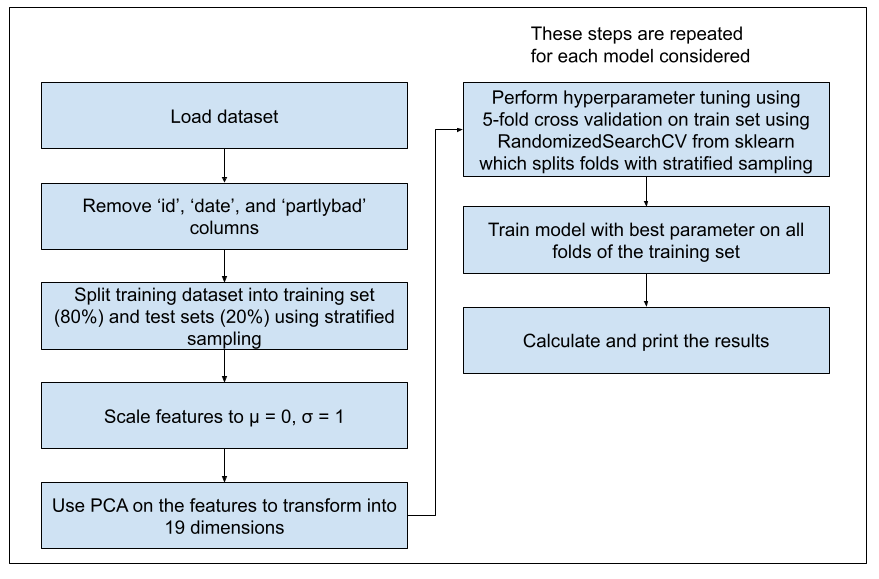
\includegraphics[scale=1.5]{pipeline}

The next step is to train the following generative and discriminative models on the datasets we have created.

\begin{enumerate}
    \item Generative model 
    
    The goal of generative models is to describe how data is created. The model relies on the Bayes theorem and uses parameters that maximizing the joint probability of P(X,Y) to trains a model. The generative models that we used are as follows:
    
    \begin{enumerate}
        \item NaiveBayes
        \item MLP classifier
    \end{enumerate}
    
    \item Discriminative model.
    
    The goal of discriminative models is to predicting the labels of the data. The model learns boundaries between classes in a dataset and trains a model using parameters that maximizing the conditional probability P(Y \textbar X). In each separate model, we set a 'class\_weight' parameter to 'balanced'. It will automatically assign class weights that are inversely proportionate to their relative frequencies. The discriminative models that we used are as follows:
    
    \begin{enumerate}
        \item Logistic Regression
        \item Logistic Regression - With Class Balanced Weights
        \item SVM
        \item SVM - With Class Balanced Weights
        \item Decision Tree
        \item Decision Tree - With Class Balanced Weights
        \item Random Forest
        \item Random Forest - With Class Balanced Weights
    \end{enumerate}
\end{enumerate}

For each model, we perform 5-fold cross-validation hyperparameter tuning. After that, the model with the best parameters is trained on train set and then evaluated on the test set for both original data and PCA.
\end{document}
 % 1.5 pgs
\chapter{Results and Discussion}
  % 2 pgs

\chapter{Conclusion}

% summarizing what we did
% describing limitations and future work
 % .5 pgs

\cleardoublepage %fixes the position of bibliography in bookmarks
\phantomsection

\renewcommand\bibname{References}
\addcontentsline{toc}{chapter}{\bibname} % This lines adds the bibliography to the ToC
\bibliographystyle{abbrv} % numbering alphabetic order
\bibliography{main}

\begin{appendices}
\myappendixtitle
\chapter{Links}

\begin{itemize}
	\item github repository: \url{https://github.com/CowKeyMan/new-particle-formation}
\end{itemize}
\end{appendices}

\end{document}
